\hypertarget{imports}{%
\subsection{Imports}\label{imports}}

\begin{lstlisting}[language=Python]
import pywt

import numpy as np
import pandas as pd

import matplotlib.pyplot as plt

from math import sqrt,log10
from sklearn.metrics import mean_squared_error

import warnings
warnings.filterwarnings('ignore')
\end{lstlisting}

\hypertarget{denoising-eeg-signals-using-discrete-wavelet-transform}{%
\subsection{Denoising EEG Signals using Discrete Wavelet
Transform}\label{denoising-eeg-signals-using-discrete-wavelet-transform}}

\textbf{Steps to denoise signals :} 1. Perform multilevel wavelet
decomposition using the wavedec() function from PyWavelets module. 2.
Select a thresholding technique. 3. Apply thresholding and reconstruct
the signal using the waverec() function from the PyWavelets module.

The Discrete Wavelet Transform splits the input signal into low pass and
high pass subbands. The low pass subband is also called the
\emph{approximation coefficient} and the high pass subband is also
called the \emph{detail coefficient} . The approximation coefficient can
be further split up on multiple levels. This is known as
\emph{Multilevel Wavelet Decomposition}.

Once we perform the multilevel wavelet decomposition we want to select a
suitable thresholding technique. For our purposes we will use the
universal thresholding technique as it is very convienient and the
universal threshold is easy to compute.

\begin{equation*}
\text{Universal Threshold} = \frac{\Bigl(\sqrt{2 \text{log(length(X))}} \Bigr) \text{median(abs(D))} }{0.6745}
\end{equation*}

where, - \textbf{X} is the signal - \textbf{D} is the set of first level
detail coefficients

Using the Universal threshold we will apply hard thresholding to the
signal, which is a type of thresholding technique where all coefficients
below the calculated threshold are reduced to 0 and all the coefficients
above the threshold value are left unchanged.

After thresholding the signal is reconstructed using the waverec()
function.

\begin{lstlisting}[language=Python]
def madev(d, axis=None):
    """ Median absolute deviation of a signal """
    return np.median(np.absolute(d))

def wavelet_denoising(x):
    c = pywt.wavedec(x,"sym18", mode="per",level = 4)
    
    sigma = (1/0.6745) * madev(c[-1])
    
    univ_thresh = sigma * np.sqrt(2 * np.log(len(x)))
    
    c[1:] = (pywt.threshold(i, value=univ_thresh, mode='hard') for i in c[1:])
    
    return pywt.waverec(c, "sym18", mode='per')


signal = pd.read_csv('data/train/subj1_data.csv')
signal = signal.drop("id", axis=1)

filtered = pd.DataFrame(wavelet_denoising(signal))

###PLOT###
plt.figure(figsize=(10, 6))
plt.plot(signal.iloc[:10000,0], label='Raw')
plt.plot(filtered.iloc[:10000,0], label='Filtered')
plt.legend()
plt.title("DWT Denoising with sym18 Wavelet", size=15)
plt.show()
\end{lstlisting}

\begin{figure}
\centering
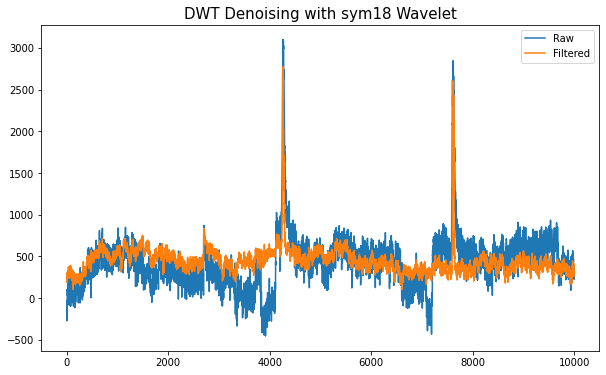
\includegraphics{denoising_files/denoising_4_0.png}
\caption{png}
\end{figure}

\hypertarget{feature-extraction-of-eeg-signals-using-discrete-wavelet-transform}{%
\subsection{Feature Extraction of EEG Signals using Discrete Wavelet
Transform}\label{feature-extraction-of-eeg-signals-using-discrete-wavelet-transform}}

The wavedec() function performs 1D multilevel Discrete Wavelet Transform
decomposition of a given signal and returns an ordered list of
coefficients arrays in the form : {[}cA\_n, cD\_n, cD\_n-1, \ldots, cD2,
cD1{]}

where n denotes the level of decomposition. The first element (cA\_n) of
the result is the approximation coefficients array and the following
elements (cD\_n - cD\_1) are detailed coefficients arrays.

Now coming to the point of different frequency bands

Discrete wavelet transform will always return only one approximation
coefficient.

If starting frequency band of the eeg waveform is 0-64 Hz then at level
=1 we will get 0-32 Hz which gives approximation coefficients \& another
band is 32-64Hz which gives the detail coefficient of the wavelet.

At level = 2, the discrete wavelet transform will return 3 frequency
bands: 1. 0-16 Hz i.e.~approximation coefficients 2. 16-32 Hz
i.e.~detail coefficients 3. 32-64 Hz i.e.~detail coefficients. and so on

Since the sampling frequency of our eeg data is 500Hz, therefore by
Nyquist-Shanon Theorem, the highest frequency in our waveform will be
250 Hz then at level =1 we will get 0-125 Hz which gives approximation
coefficients \& another band is 125-250Hz which gives the detail
coefficient of the wavelet.

Therefore at level = 5, the discrete wavelet transform will return 3
frequency bands: 1. 0 - 7.8125 Hz i.e.~approximation coefficients 2.
7.8125 - 15.625 Hz \textasciitilde{} Alpha Frequency Band 3. 15.625
-31.25 Hz \textasciitilde{} Beta Frequency Band 4. 31.25 - 62.5 Hz 5.
62.5 - 125 Hz 6. 125 - 250 Hz

The aim is to extract Alpha and Beta frequencies as they correspond to
motor function.

\begin{lstlisting}[language=Python]
def FEdwt(s):
    coefli = pywt.wavedec(s,"sym18", mode="per", level=5)
    return coefli

cli = FEdwt(filtered)

i = 5
for c in cli[1:3:]:
    d = pd.DataFrame(pywt.idwt(None, c,"sym18", mode="per"))
    
    ###PLOT###
    plt.figure(figsize=(10, 6))
    plt.plot(d.iloc[:], label='')
    plt.title(f"Level {i} details", size=15)
    plt.show()
    i-=1
\end{lstlisting}

\begin{figure}
\centering
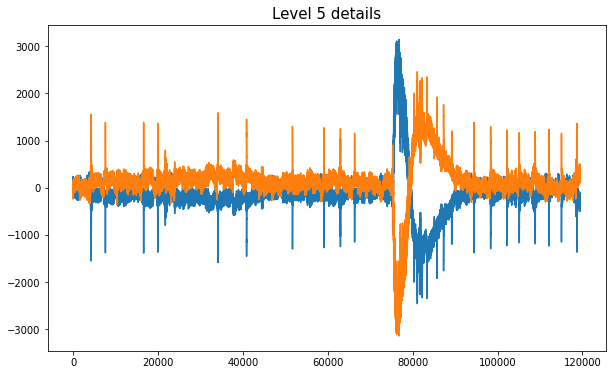
\includegraphics{denoising_files/denoising_7_0.png}
\caption{png}
\end{figure}

\begin{figure}
\centering
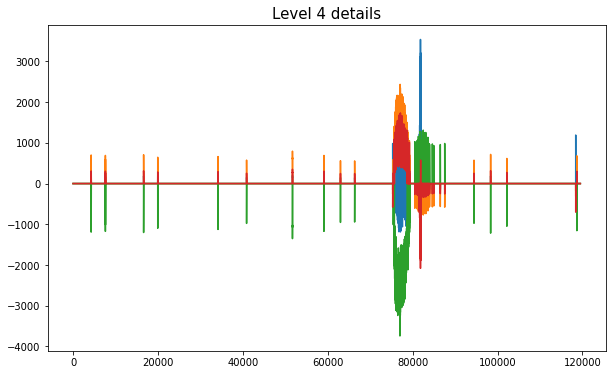
\includegraphics{denoising_files/denoising_7_1.png}
\caption{png}
\end{figure}
